\documentclass[11pt]{article}
\usepackage[utf8]{inputenc}
\usepackage[ngerman]{babel}
\usepackage{amsmath}
\usepackage{amsfonts}
\usepackage{amssymb}
\usepackage{lmodern}
\usepackage{enumitem}
\usepackage{graphicx}
\usepackage[top=2cm,bottom=2cm]{geometry}
\date{}
\begin{document}
\title{\textbf{Entwicklung und Anwendung von Methoden des
Maschinellen Lernens zum In-situ-Prozessmonitoring
beim 3D-Druck}}
\maketitle
\noindent
Prozessverständnis sowie daraus abgeleitete Prozessoptimierung können zur Verbesserung
der Maßhaltigkeit sowie zur Beschleunigung des gesamten Produktionsprozesses bei additiven
Fertigungstechnologien beitragen. In-situ-Monitoring der Materialzustände bei generativen
Herstellungsprozessen soll neue Erkenntnisse über Ursache-Wirk-Zusammenhänge bei dem
Fertigungsprozess ermöglichen. Das Thema adressiert die Entwicklung und Erprobung einer
datengetriebenen Vorgehensweise zur Ermittlung qualitätsgerechter Prozessanpassungen basierend
auf einer Kombination von optischen Diagnosetechniken mit Methoden des Maschinellen
Lernens. Die Arbeit kann als Beleg- oder Diplomarbeit belegt werden.\\

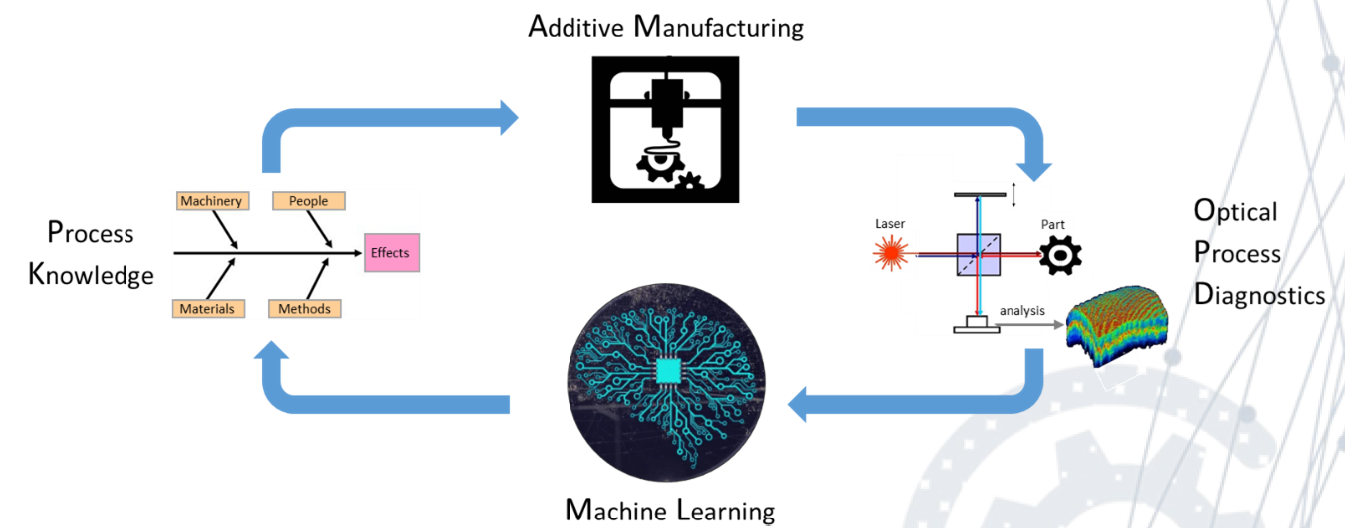
\includegraphics[scale=0.4]{DA.png}
\\

\noindent
\textbf{Erforderliche Kenntnisse und Fertigkeiten des Studenten:}
\begin{itemize}[itemsep=0pt,parsep=0pt]
\item Grundkenntnisse der Steuerungstechnik (SPS-Programmierung, etc.)
\item Grundkenntnisse des Maschinellen Lernens
\item Kenntnisse in CAD-Konstruktion
\end{itemize}

\noindent
\textbf{Aufgabenschwerpunkte:}
\begin{itemize}[itemsep=0pt,parsep=0pt]
\item Entwicklung und Implementierung von Sensorik an einer Bearbeitungsmaschine
\item Durchführung von Experimenten
\item Analyse und Auswertung der Ergebnisse
\end{itemize}

\end{document}

